%!TEX program = xelatex
\documentclass[dvipsnames, svgnames,a4paper,11pt]{article}
% ----------------------------------------------------- 
%	加边框的命令
%	参考:https://tex.stackexchange.com/questions/531559/how-to-add-the-page-border-for-first-two-pages-in-latex
\usepackage{tikz}
\usetikzlibrary{calc}
\usepackage{eso-pic}
\AddToShipoutPictureBG{%
\begin{tikzpicture}[overlay,remember picture]
\draw[line width=0.6pt] % 边框粗细
    ($ (current page.north west) + (0.6cm,-0.6cm) $)
    rectangle
    ($ (current page.south east) + (-0.6cm,0.6cm) $); % 边框位置
\end{tikzpicture}}


\usepackage{xcolor}
\definecolor{c1}{HTML}{070F94} % 目录颜色 原版为2752C9 紫灰色535AAA 蓝紫色0B0DB7 深蓝色070F94 湖绿色219394 松石灰绿086173
\definecolor{c2}{HTML}{E20129} % 引用颜色 原版\definecolor{c2}{RGB}{190,20,83} 橙色F24729

\usepackage{ctex}
\usepackage[top=28mm,bottom=28mm,left=15mm,right=15mm]{geometry}
\usepackage{hyperref} 
\hypersetup{
	colorlinks,
	linktoc = section, % 超链接位置,选项有section, page, all
	linkcolor = c1, % linkcolor 目录颜色
	citecolor = c1  % citecolor 引用颜色
}
\usepackage{amsmath,enumerate,multirow,float}
\usepackage{tabularx}
\usepackage{tabu}
\usepackage{subfig}
\usepackage{fancyhdr}
\usepackage{graphicx}
\usepackage{wrapfig}  
\usepackage{physics}
\usepackage{appendix}
\usepackage{amsfonts}

%
\usepackage{tcolorbox}
\tcbuselibrary{skins,breakable}
\newtcolorbox{tbox}[2][]{
    colframe=black!70!,
    breakable,
    enhanced,
	boxrule =0.5pt,
    title = {#2},
    fonttitle = \large\kaishu\bfseries,
	drop fuzzy shadow,
    #1
}
\newtcolorbox[auto counter,number within=section]{question}[1][]{
  top=2pt,bottom=2pt,arc=1mm,
  boxrule=0.5pt,
%   frame hidden,
  breakable,
  enhanced, %跨页后不会显示下边框
  coltitle=c1!80!gray,
  colframe=c1,
  colback=c1!3!white,
  drop fuzzy shadow,
  title={思考题~\thetcbcounter:\quad},
  fonttitle=\bfseries,
  attach title to upper,
  #1
}

% ---------------------------------------------------------------------
%	利用cleveref改变引用格式,\cref是引用命令
\usepackage{cleveref}
\crefformat{figure}{#2{\textcolor{c2}{Figure #1}}#3} % 图片的引用格式
\crefformat{equation}{#2{(\textcolor{c2}{#1})}#3} % 公式的引用格式
\crefformat{table}{#2{\textcolor{c2}{Table #1}}#3} % 表格的引用格式


% ---------------------------------------------------------------------
%	页眉页脚设置
\fancypagestyle{plain}{\pagestyle{fancy}}
\pagestyle{fancy}
\lhead{\kaishu 中山大学物理与天文学院基础物理实验\uppercase\expandafter{\romannumeral2}} % 左边页眉,学院 + 课程
\rhead{\kaishu 实验报告By黄罗琳} % 右边页眉,实验报告标题
\cfoot{\thepage} % 页脚,中间添加页码


% ---------------------------------------------------------------------
%	对目录、章节标题的设置
\renewcommand{\contentsname}{\centerline{\huge 目录}}
\usepackage{titlesec}
\usepackage{titletoc}
% \titleformat{章节}[形状]{格式}{标题序号}{序号与标题间距}{标题前命令}[标题后命令]
\titleformat{\section}{\centering\LARGE\songti}{}{1em}{}

% ---------------------------------------------------------------------
%   listing代码环境设置
\usepackage{listings}
\lstloadlanguages{python}
\lstdefinestyle{pythonstyle}{
backgroundcolor=\color{gray!5},
language=python,
frameround=tftt,
frame=shadowbox, 
keepspaces=true,
breaklines,
columns=spaceflexible,                   
basicstyle=\ttfamily\small, % 基本文本设置,字体为teletype,大小为scriptsize
keywordstyle=[1]\color{c1}\bfseries, 
keywordstyle=[2]\color{Red!70!black},   
stringstyle=\color{Purple},       
showstringspaces=false,
commentstyle=\ttfamily\scriptsize\color{green!40!black},%注释文本设置,字体为sf,大小为smaller
tabsize=2,
morekeywords={as},
morekeywords=[2]{np, plt, sp},
numbers=left, % 代码行数
numberstyle=\it\tiny\color{gray}, % 代码行数的数字字体设置
stepnumber=1,
rulesepcolor=\color{gray!30!white}
}




% ---------------------------------------------------------------------
%	其他设置
\def\degree{${}^{\circ}$} % 角度
\graphicspath{{./images/}} % 插入图片的相对路径
\allowdisplaybreaks[4]  %允许公式跨页 
\usepackage{lipsum}
\usepackage{adjustbox}
\usepackage{tabularray}
\usepackage{array}
%\usepackage{mathrsfs} % 字体
%\captionsetup[figure]{name=Figure} % 图片形式
%\captionsetup[table]{name=Table} % 表格形式
\begin{document}
	
	% 实验报告封面	
	% 顶栏
	\begin{table}
		\renewcommand\arraystretch{1.7}
		\begin{tabularx}{\textwidth}{
				|X|X|X|X
				|X|X|X|X|}
			\hline
			\multicolumn{2}{|c|}{预习报告}&\multicolumn{2}{|c|}{实验记录}&\multicolumn{2}{|c|}{分析讨论}&\multicolumn{2}{|c|}{总成绩}\\
			\hline
			\LARGE25 & & \LARGE25 & & \LARGE30 & & \LARGE80 & \\
			\hline
		\end{tabularx}
	\end{table}
	% ---
	
	% 信息栏
	\begin{table}
		\renewcommand\arraystretch{1.7}
		\begin{tabularx}{\textwidth}{|X|X|X|X|}
			\hline
			年级、专业: & 2022级 物理学 &组号: & 实验班2\\
			\hline
			姓名: & 黄罗琳、徐靖博   & 学号: &   22344001、22344004\\
			\hline
			实验时间: & 2024/6/5 & 教师签名: & \\
			\hline
		\end{tabularx}
	\end{table}
	% ---
	
	% 大标题
	\begin{center}
		\LARGE 塞曼效应 \quad 实验报告
	\end{center}
	% ---
	
	% 注意事项
	
	% 基本
	\textbf{【实验报告注意事项】}
	\begin{enumerate}
		\item 实验报告由三部分组成:
		\begin{enumerate}
			\item 预习报告:课前认真研读实验讲义,弄清实验原理;实验所需的仪器设备、用具及其使用、完成课前预习思考题;了解实验需要测量的物理量,并根据要求提前准备实验记录表格(可以参考实验报告模板,可以打印)。\textcolor{red}{\textbf{(20分)}}
			\item 实验记录:认真、客观记录实验条件、实验过程中的现象以及数据。实验记录请用珠笔或者钢笔书写并签名(\textcolor{red}{\textbf{用铅笔记录的被认为无效}})。\textcolor{red}{\textbf{保持原始记录,包括写错删除部分,如因误记需要修改记录,必须按规范修改。}}(不得输入电脑打印,但可扫描手记后打印扫描件);离开前请实验教师检查记录并签名。\textcolor{red}{\textbf{(30分)}}
			\item 数据处理及分析讨论:处理实验原始数据(学习仪器使用类型的实验除外),对数据的可靠性和合理性进行分析;按规范呈现数据和结果(图、表),包括数据、图表按顺序编号及其引用;分析物理现象(含回答实验思考题,写出问题思考过程,必要时按规范引用数据);最后得出结论。\textcolor{red}{\textbf{(30分)}}
		\end{enumerate}
		\textbf{实验报告就是将预习报告、实验记录、和数据处理与分析合起来,加上本页封面。\textcolor{red}{(80分)}}
		\item 每次完成实验后的一周内交\textbf{实验报告}(特殊情况不能超过两周)。
		
		
	\end{enumerate}
	
	% 安全
	\textbf{【实验安全注意事项】}	
	\begin{enumerate}
		\item 不要用手直接触摸光学部件的光学表面,如果有污染,请用专用的清洁液和清洁布或者擦镜纸清洁。
		\item F-P 标准具已在出厂前进行校准,请勿自行随意调节三颗螺钉,如需调整,请在实验老师指导下进行。
		\item 为避免缩短笔形汞灯使用寿命,请勿频繁开关电源开关。笔形汞灯插入槽内后严禁左右晃动,以免破碎。
		\item 避免长时间对电磁线圈进行大电流供电,温度较高,请勿触摸。
		\item 每次实验结束后将电流调至零后再关掉电源。
	\end{enumerate}
	% 目录
	\clearpage
	\tableofcontents
	\clearpage

	
	
	
	% 预习报告	
	
	% 小标题
	\setcounter{section}{0}
	\section{塞曼效应\quad\heiti 预习报告}
	% ---
	
	% 实验目的
	\subsection{实验目的}
	\begin{enumerate}
		\item 通过观察原子谱线在外磁场中的分裂现象,加深对电子“自旋”、“两个角动量的耦合”、“两个电子之间的 LS 耦合”、“角动量守恒”、“多电子原子和电子组态”、“能级跃迁”、“选择定则”等概念的理解,验证原子具有磁矩及其空间取向的量子化,进一步认识原子的内部结构;
		\item 用 F-P 干涉仪观察汞(Hg)原子 546.1nm 谱线在外磁场中的分裂现象(即“反常塞曼效应”),测量电子的荷质比 e/m;
		\item 验证光子具有角动量及角动量守恒定律,了解光的偏振理论及其产生机制,学习偏振片的原理及使用方法。
	\end{enumerate}
	% ---
	
	% 仪器用具
	\subsection{仪器用具}
\begin{table}[htbp]
    \centering
    \renewcommand\arraystretch{1.6}
    \begin{tabular}{p{0.05\textwidth}|p{0.20\textwidth}|p{0.05\textwidth}|p{0.5\textwidth}}
        \hline
        编号 & 仪器用具名称 & 数量 & 主要参数(型号,测量范围,测量精度等) \\
        \hline
        1 & 塞曼效应 & 1 & BEX-8501 \\
        2 & 电磁体(带电源) & 1 & 可通过调节激励电流大小改变磁场的大小 \\
        3 & 磁感应强度测量仪 & 1 & 含金属探针 \\
        4 & 汞放电管 & 1 & \\
        5 & 滤光片 & 1 & 能通过 546.1nm 及其自由光谱范围内的“单色光” \\
        6 & 法布里-珀罗标准具 & 1 &  \\
        7 & 偏振片 & 1 & 可以通过 0° 刻度线方向上的线偏振光\\
        8 & 数字图像采集器 & 1 & 包含望远镜和 CCD \\
        9 & 台式电脑 & 1 & 安装有“塞曼效应实验分析 VCH5.0”软件,用以分析实验数据 \\
        \hline
    \end{tabular}
\end{table}
	% ---
	
	% 原理概述
	\subsection{原理概述}
	\subsubsection{电子的磁矩——轨道磁矩和自旋磁矩}

	\begin{enumerate}
		\item 电子的轨道磁矩

			\[
				\mu_l = \sqrt{l(l+1)}\frac{e \hbar}{2 m_e} \equiv \sqrt{l(l+1)}\mu_B \quad l=0,1,2,\cdots , n-1	
			\]

			\[
				\mu_{l,z} = m_l \hbar \cdot \frac{e}{2 m_e} = m_l \mu_B \quad m_l = 0,\pm 1,\cdots ,\pm l	
			\]

			其中$\mu_B \equiv \frac{e \hbar}{2 m_e} =0.9274 \times 10^{23} A\cdot m^2$


		\item 电子的自旋 及自旋磁矩
		
			电子除了轨道角动量外,还有自旋运动,电子的自旋是一种固有的内在属性,电子自旋角动量及其 z 方向分量大小的可能取值为:

			\[
				S = \sqrt{s(s+1)}\hbar \quad s = \frac{1}{2}	
			\]

			\[
				S_z = m_s \hbar \quad m_s = \pm \frac{1}{2}	
			\]


			由电子自旋运动产生的自旋磁矩,其方向及大小为:

			\[
				\vec{\mu_s} = -2 \gamma \vec{S}
			\]

			\[
				\mu_s = 2\sqrt{s(s+1)}\mu_B \quad s = \frac{1}{2}
			\]

			\[
				\mu_{s,z} = 2 m_s \mu_B \quad m_s = \pm \frac{1}{2}
			\]

		\item 磁矩在外磁场 中的势能
				
			在电磁学中,磁矩为的系统,在外磁场中的势能为:
			\[
				U = - \vec{\mu} \cdot \vec{B}
			\]	
				
	\end{enumerate}


\subsubsection{两个角动量的耦合(叠加)}

	\begin{enumerate}
		\item 同一个电子的情况

			同一个电子,其轨道角动量L和自旋角动量S的叠加或耦合。此即所谓的“自旋—轨道耦合”。自旋—轨道耦合本质上是电子自旋(内禀)磁矩与电子轨道运动产生的磁场之间的相互作用,“自旋—轨道耦合”是导致氢原子和碱金属光谱双线结构的主要原因:

				\[
					\vec{J}=\vec{L}+\vec{S}	
				\]

		\item 不同电子之间的耦合

			\begin{itemize}
				\item LS 耦合:即电子1的$L_1$和电子2的$L_2$耦合成$\vec{L}=\vec{L_1}+\vec{L_2}$,电子1的$S_1$和电子2的$S_2$耦合成$\vec{S}=\vec{S_1}+\vec{S_2}$,然后系统的总轨道角动量$\vec{L}$和总自旋角动量$\vec{S}$再耦合生成系统的总角动量$\vec{J}$
				
				\item jj耦合:即电子1的$L_1$和$S_1$耦合成$\vec{J_1}=\vec{L_1}+\vec{S_1}$,即电子2的$L_2$和$S_2$耦合成$\vec{J_2}=\vec{L_2}+\vec{S_2}$,然后电子1的总角动量$\vec{J_1}$和电子2的总角动量$\vec{J_2}$再耦合成系统的总动量$\vec{J}$。
			\end{itemize}

			
	\end{enumerate}



\subsubsection{电子的总磁矩 及其在外磁场中的势能}

	\begin{enumerate}
		\item 电子的总磁矩
		
			总磁矩$\vec{\mu_j}$及其大小的一般表达式可写成:
				\[
					\mu_j = -\sqrt{j(j+1)}g_j \mu_B
				\]

			总磁矩$\vec{\mu_j}$在z方向上分量的大小为:
				\[
					\mu_{j,z} = - m_j g_j \mu_B	
				\]

			朗德因子的一般表达式为:
				\[
					g_j=\frac{3}{2}+\frac{s\left(s+1\right)-l\left(l+1\right)}{2j\left(j+1\right)}	
				\]

		\item 弱外磁场和强外磁场的区别
		
			\begin{itemize}
				\item 弱外磁场:当外磁场$B_{ext}$的场强远远小于原子内部磁场$B_{int}$的场强,即为弱外磁场时,这时自旋—轨道耦合占主导,电子的总角动量J是守恒量,但总轨道角动量L和总自旋角动量S均不守恒, 系统的守恒量(好量子数)为$J^2,J_z,L^2,S^2\left(n,\ L,\ J,\ mj\right)。$
				\item 强外磁场: 自旋—轨道耦合变得次要,电子磁矩(分为轨道磁矩和自旋磁矩)与外磁场$B_{ext}$的相互作用则占主导。系统的总轨道角动量L和总自旋角动量S不再耦合成总角动量J(仍然可通过$\vec{J}=\vec{L}+\vec{S}$计算总角动量,但此时的总角动量是非守恒量, (24)至(28)式在强外磁场的情况下不适用),此时系统的守恒量(好量子数)为$L^2,L_Z,\ \ S^2,\ {\ S}_z\left(n,\ L,\ ml,\ ms\right)$。
			\end{itemize}
		
		\item 电子总磁矩 在外磁场 中的势能
		
			可得汞原子的总磁矩$\vec{\mu_j}$在沿着 z 轴方向的外磁场B中的势能为:
			\[
				U=-\mu_J \cdot B=m_jg_j\mu_B B	
			\]


	\end{enumerate}





\subsubsection{汞原子谱线在外磁场 中的能级分裂}

	\begin{enumerate}
		\item 原子谱线在外磁场中的分裂

			当原子处于磁感应强度为B的外磁场中时,原子磁矩与磁场相互作用,使原子系统附加了势能$\Delta E=U$,此时原子的能级将分裂为2J+1层,各层能量为:
			\[
				E = E_0 +m_J g_J \mu_B B
			\]

			又设频率为$\nu$的光子是由原子从能级E2跃迁到能级E1所产生,即有:
			\[
				h\nu = E_2 - E_1 = E_{20} - E_{10} + (m_2 g_2 -m_1 g_1)\mu_B B	
			\]

			分裂后的谱线和原来谱线之间的频率差为:
			\[
				\Delta \nu = (m_2 g_2 -m_1 g_1)\mu_B B / h
			\]

			波数差(波数定义$\widetilde{\upsilon}=1/\lambda$):
			\[
				\Delta \tilde{\nu} = \frac{(m_2 g_2 - m_1 g_1)eB}{4 \pi m c} 	
			\]

		\item 汞原子 546.1nm 谱线的量子数及朗德因子 的计算
		
			谱线是汞原子的外层(两个)电子从能级(组态)6s7s到6s7p的跃迁而产生的。 

				\begin{figure}[H]
					\centering
					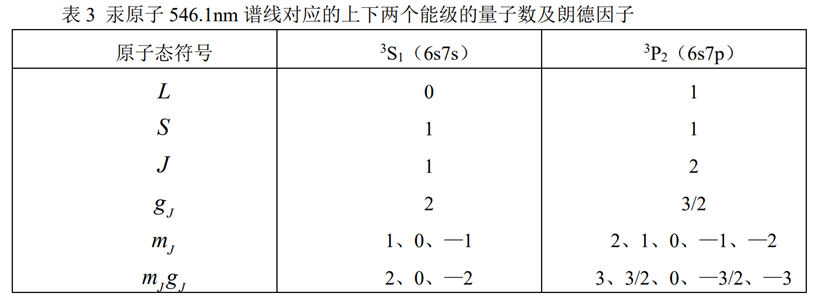
\includegraphics[width=0.8\textwidth]{graph1-6.png}
					\label{fig:graph1-6}
				\end{figure}

				\begin{figure}[H]
					\centering
					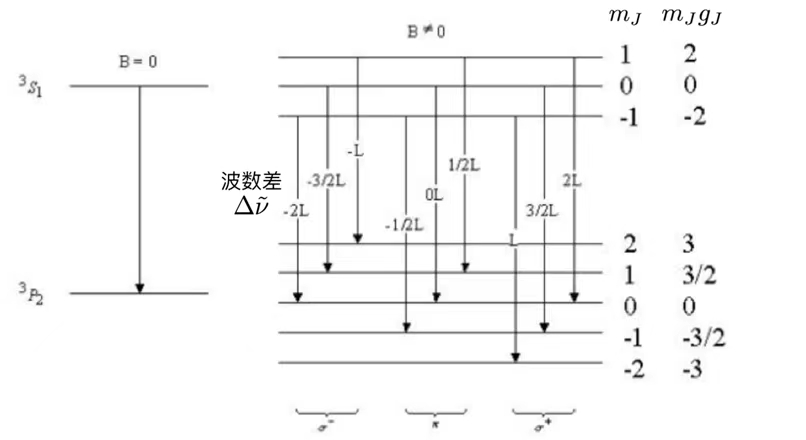
\includegraphics[width=0.8\textwidth]{graph1-7.jpg}
					\label{fig:graph1-7}
				\end{figure}
			
		\item 塞曼效应观测中的偏振效应——$\sigma^\pm$偏振(垂直于磁场)和$\pi$偏振(平行于磁场)
		
			若有$\Delta m = 1$,将观察到$\sigma^+$左旋偏振光,若$\Delta m = -1$,将观察到$\sigma^-$右旋偏振光,若$\Delta m = 0$,则为$\pi$偏振。
	\end{enumerate}	





\subsubsection{基本测量仪器介绍}

	\begin{enumerate}
		\item 法布里—珀罗标准具

			F-P 标准具由平行放置的两块平面板组成的, 在两板相对的平面上镀薄银膜和其他有较高反射系数的薄膜, 若两平行的镀银平面的间隔不可以改变,则称该仪器为“法布里—珀罗干涉仪”。由于两镀膜面平行,若使用扩展光源,则产生等倾干涉条纹。具有相同入射角的光线在垂直于观察方向的平面上的轨迹是一组同心圆。若在光路上放置透镜,则在透镜焦平面上得到一组同心圆环图样。 在透射光束中,相邻光束的光程差为:
			\[
				\Delta = 2 n d cos \phi	
			\]

			产生亮条纹的条件为:
			\[
				2 n d cos \phi = K \lambda
			\]

			其中K为干涉条纹级数,$\lambda$为入射光波长。

			标准具的两个特征参量是自由光谱范围和分辨本领。
				
				\begin{itemize}
					\item 自由光谱范围:同一光源发出的具有微小波长差的单色光$\lambda_1$和$\lambda_2$,入射后将形成各自的圆环系列。对同一级的干涉条纹,波长大的干涉圆环直径小。对于某单色光来说,越靠中心处的干涉条纹的级数 K 越大。
					
					如果$\lambda_1$和$\lambda_2$的波数差逐渐增大,使得$\lambda_1$的第$m$级亮纹与$\lambda_2$的第$m - 1$级亮纹重合,则有
					\[
						2 n d \cos \theta = m \lambda _1 = (m - 1)\lambda_2	
					\]

					得出$\Delta \lambda = \lambda _2 - \lambda_1 = \frac{\lambda_2}{m}$

					由于大多数情况下,$\cos \theta \approx 1$,可得到$m = \approx \frac{2 n d}{\lambda_1}$,得
					\[
						\Delta \lambda = \frac{\lambda_1 \lambda_2}{2 n d} \approx \frac{\lambda^2}{2 n d}	
					\]

					它表明在 F-P 干涉仪中,当给定两平面间隔d后,入射光波长在$\lambda \pm \Delta \lambda$内不会发生干涉圆环重叠。

					\item 分辨本领:对于F-P标准具,它的分辨本领为$\frac{\Delta \lambda}{\lambda} = K N$,K为干涉级次,N为精细度, 它的物理意义是在相邻两个干涉级之间能分辨的最大条纹数。N依赖于平板内表面反射膜的反射率R:
					\[
						N = \frac{\pi \sqrt{R}}{1 -1R}	
					\]

					反射率R越高,精细度N就越高,仪器能分辨开的条纹数就越多。

				\end{itemize}

		\item 波数差与圆环直径之间的关系
		
			通过测量干涉环的直径就可以测量各分裂谱线的波长或波长差。

			如图所示,出射角为$\theta$的的圆环直径D与透镜焦距f间的关系为$\tan{\theta}=\frac{D}{2f}$,对于近中心的圆环$\theta$很小,可以认为$\theta\approx\sin{\theta}\approx\tan{\theta}$,于是有:
			\[
				cos\theta = 1 - 2 \sin^2\frac{\theta}{2} \approx 1 - \frac{\theta^2}{2} = 1 - \frac{D^2}{8f^2}	
			\]

			\begin{figure}[H]
				\centering
				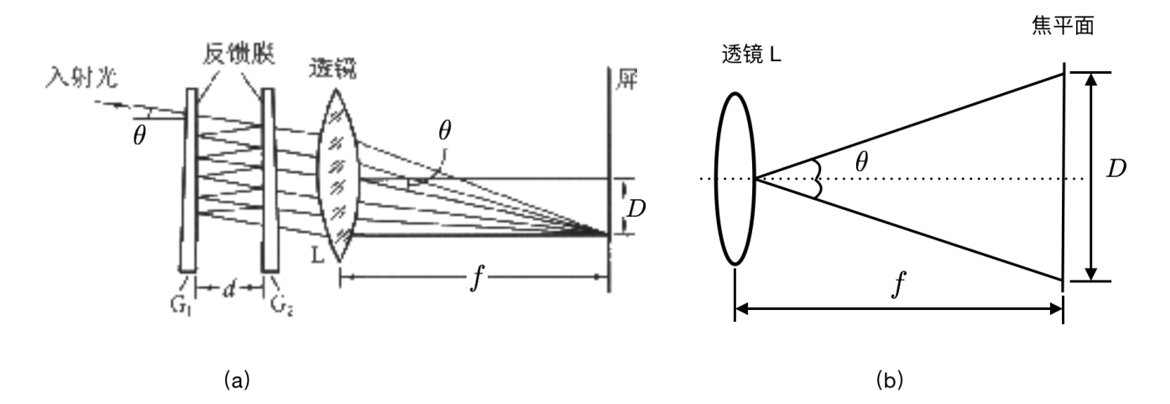
\includegraphics[width=0.8\textwidth]{graph1-9.png}
				\caption{法布里一珀罗(F-P)标准具光路图(图中的透镜指的是望远镜里的透镜)}
		
			\end{figure}

			\[
				2 n d \cos \theta = 2 n d (1 - \frac{D^2}{8f^2}) = K \lambda	
			\]

			由上式可推出同一波长$\lambda$相邻两级$K$和$K - 1$级圆环直径的平方差为
			\[
				\Delta D^2 = D^2_{K-1} - D^2_{K} = \frac{4 f^2 \lambda}{n d}	
			\]

			设不同波长$\lambda$和$\lambda_{\alpha}$的第K级干涉圆环直径分别为$D_K$和$D_{\alpha}$
			\[
				\lambda - \lambda_\alpha = \frac{nd}{4 f^2 K}(D^2_\alpha - D^2_K) = (\frac{D^2_\alpha - D^2_K}{D^2_{K-1} - D^2_{K}})\frac{\lambda}{K}	
			\]

			得出波长差为:
			\[
				\Delta \lambda = \frac{\lambda^2}{2 n d}(\frac{D^2_\alpha - D^2_K}{D^2_{K-1} - D^2_{K}})
			\]
			
			波数差为:
			\[
				\Delta \tilde{\nu} = \frac{1}{2 n d}(\frac{D^2_\alpha - D^2_K}{D^2_{K-1} - D^2_{K}})
			\]

		\item 通过塞曼效应计算电子荷质比e/m
		
			本实验只研究反常塞曼效应的线偏振$\pi$的谱线。
			\[
				\frac{e}{m} = \frac{4\pi c}{n d B}(\frac{D^2_\alpha - D^2_K}{D^2_{K-1} - D^2_{K}})
			\]
			
			若已知$d$和$B$,从塞曼分裂中测量出各环的直径,就可以计算出荷质比。
	\end{enumerate}

	% ---
	
	
	
	% 实验前思考题
	\subsection{实验预习题}
	
	% 思考题1
	\begin{question}
		光子是否具有角动量?试描述光子角动量方向与光的偏振方向之间的关系。
光子具有角动量,包括自旋角动量(内禀角动量)和轨道角动量。

	\end{question}
	光子具有自旋角动量和轨道角动量;光子自旋角动量$\pm\hbar$分别对应左旋、右旋圆偏振光。

	
	\subsection*{光子的自旋角动量}
	
	光子的自旋角动量 $S$ 与其偏振方向有关。光子的偏振描述的是电场矢量 $\mathbf{E}$ 振动的方向。对于线偏振光,电场矢量在特定方向上振动。
	
	对于圆偏振光(左旋或右旋),电场矢量的振动方向会绕传播方向旋转。左旋圆偏振光(逆时针旋转)对应自旋角动量为 $+\hbar$,而右旋圆偏振光(顺时针旋转)对应自旋角动量为 $-\hbar$。
	
	用数学表达式表示:
	

$$	\mathbf{S} = \pm \hbar \hat{\mathbf{k}}$$

	
	其中 $\hat{\mathbf{k}}$ 是光子的传播方向的单位矢量,$+\hbar$ 对应左旋圆偏振,$-\hbar$ 对应右旋圆偏振。
	
	\subsection*{光子的轨道角动量}
	
	光子还可以携带轨道角动量 $L$,这与光束的相位前沿形状相关。轨道角动量可以由螺旋相位前沿或光束中的涡旋结构引起。轨道角动量的大小可以是 $\ell \hbar$,其中 $\ell$ 是一个整数。
	
	总角动量 $J$ 是自旋角动量 $S$ 和轨道角动量 $L$ 的矢量和:
	
	$$
	\mathbf{J} = \mathbf{L} + \mathbf{S}.
	$$
	
	\subsection*{自旋角动量与偏振方向的关系}
	
	光子的自旋角动量方向与偏振方向之间的关系可以总结如下:
	
	\begin{itemize}
		\item 对于线偏振光,自旋角动量为零,因为电场矢量固定在一个平面内振动。
		\item 对于圆偏振光,自旋角动量方向与光的传播方向($\hat{\mathbf{k}}$)一致(左旋)或相反(右旋)。
	\end{itemize}
	
	\subsection*{塞曼效应中的角动量守恒}
	
	在塞曼效应中,系统的角动量(自旋)需要守恒。不同的跃迁($\Delta m = 0, \pm1$)会对应不同的光子自旋状态,从而导致光表现为不同的偏振态。
	
	\begin{itemize}
		\item 当 $\Delta m = \pm1$ 时,跃迁会导致发射的光子具有圆偏振($\sigma$光),因为光子的自旋角动量改变了 $\pm1$。
		\item 当 $\Delta m = 0$ 时,跃迁对应的光子是线偏振($\pi$光),因为在这种情况下光子的自旋角动量没有变化。
	\end{itemize}
	
	因此,光子的自旋角动量与偏振方向的关系可以通过理解偏振状态以及在特定物理效应(如塞曼效应)中的角动量守恒来确定。
	
	% 思考题2
	\begin{question}
		用同一级条纹的内外圈分别计算电子的荷质比,结果一样吗?试简述原因。
	\end{question}
	电子的荷质比($e/m$)是通过观察电子在磁场中运动时的轨迹来计算的。在等倾干涉中,通过测量内外圈的条纹直径,可以间接计算出电子的荷质比。

在等倾干涉中,不同条纹表示不同的光程差,这意味着它们的厚度不同。内外圈的条纹对应的厚度差异会影响测量结果。假设我们有两个同一级条纹,其内圈直径为 $D_1$ 和外圈直径为 $D_2$,它们之间的平方差为 $\Delta$。 

对于同一级条纹,若我们用内圈直径 $D_1$ 和外圈直径 $D_2$ 分别计算电子的荷质比 $e/m$,结果会不同。这是因为圆环并不是等厚的,随着条纹级数 $N$ 的增加,圆环的厚度变化($\delta D$)会影响直径的测量。具体来说,随着级数的增加,圆环的厚度变化导致直径的变化,从而使得计算的结果有所偏差。

通过以下推导可以看出这种影响:

\begin{align*}
\Delta &= D_2^2 - D_1^2 \\
\Delta' &= (D_2 + \delta D_2)^2 - (D_1 + \delta D_1)^2 \\
\Delta' &\approx \Delta + 2\delta D (D_2 - D_1) \\
\Delta' &\approx \Delta \left(1 + \frac{2 \delta D}{D_1 + D_2}\right)
\end{align*}

这表明,内外圈的条纹直径由于厚度变化引起的误差导致计算出的电子荷质比不同。这种误差随着圆环厚度的变化而变化,因此结果不一样。

综上所述,内外圈条纹的测量结果不同,因为它们对应的厚度不同,厚度变化影响了条纹的直径,进而影响了荷质比的计算结果。

	% 思考题3
	\begin{question}
		请利用(20)至(23)式,计算汞原子$^3\mathcal{S}_1$ (6s7s)和$^3\mathcal{P}_2$ (6s7p)能级所对应的量子数(见表
1),并给出详细的计算过程。
	\end{question}
	
$$^3S_1\colon l_1=l_2=0,L=0;s_1=s_2=\frac12,S=1;L=0.$$
$$^3P_2\colon l_1=0,l_2=1,L=1;s_1=s_2=\frac12,S=1;L=2.$$
\begin{question}
	请利用(2)、(8)和(20)式,并结合 和 (注意此时的是图 5 中的 ,详细见脚注 22),导出朗德因子的一般表达式(28)式,并给出详细的推导过程。
\end{question}
	其中(2)式为:
	$$\vec{\mu}_{l}=e/\left(\frac{2\pi r}{v}\right)\cdot\pi r^{2}\vec{e}_{n}=-\frac{e}{2m_{e}}\cdot m_{e}rv\vec{e}_{n}=-\frac{e}{2m_{e}}\vec{L}\equiv-\gamma\vec{L}$$

	(8)式为:
$$\vec{\mu}_s=-2\gamma\vec{S}$$
	\begin{align*}
		\mu_{J} &= \mu_{s} \cos \alpha + \mu_{L} \cos \beta \\
		\cos \alpha &= \frac{S^2 + J^2 - L^2}{2SJ} \\
		\cos \beta &= \frac{L^2 + J^2 - S^2}{2LJ} \\
		\mu_{J} &= g_{J} \sqrt{J(J+1)} \\
		\mu_{S} &= \sqrt{S(S+1)} \\
		\mu_{L} &= \sqrt{L(L+1)}
		\end{align*}
		\begin{align*}
			g_j &= \frac{g_l(j^2 + l^2 - s^2)}{2j^2} + \frac{g_S(j^2 + S^2 - l^2)}{2j^2} \\
			g_j &= \frac{3}{2} + \frac{1}{2} \left(\frac{l^2 - s^2}{j^2}\right) \\
			&= \frac{3}{2} + \frac{1}{2} \frac{l(l+1) - s(s+1)}{j(j+1)}
			\end{align*}
	
			\begin{question}
				5请利用单电子情况下的(36)式,并结合钠双黄线的平均波长及其波长差($\lambda_1=589.$Onm, $\lambda_{2}=589.6$nm),估算一下钠原子内部的磁感应强度$B_int$的值(提示:单电子情况下,两谱线的能级差为势能的两倍,即有$\Delta E=2\Delta U=2\mu_BB$;另需要利用到光子波长和频率之间的关系式。答案:钠原子内部的磁感应强度$B_{int}$的值为 18.5T)。
			\end{question}

			由 $U = m_J g_J \mu_B$,单电子 $\Delta m = 1$,$g_J = 2$ 可得:

\begin{equation}
2\mu_B B_{\text{int}} = hc \Delta \frac{\Delta \lambda}{\lambda_1 \lambda_2}
\end{equation}

\begin{equation}
B_{\text{int}} = 18.5\, \text{T}
\end{equation}



\begin{question}
	请结合第 5 题的计算结果,说明弱外磁场$B_ext\ll B_{int}$成立时弱外磁场$B_ext$的取值范围,并确认本
	实验中电磁体的磁感应强度符合弱外磁场$B_ext\ll B_{int}$条件。
\end{question}
由思考题 5 可知,

\begin{equation}
B_{ext} \leq 18.5\, \mathrm{T} = 185000\, \mathrm{Gs}
\end{equation}

实验中磁场强度为 $3000\, \mathrm{Gs} \sim 185000\, \mathrm{Gs}$,符合弱外磁场条件。

\begin{equation}
B_{ext} \ll B_{int}
\end{equation}



\begin{question}
	 请结合力与势能的关系式$\vec{F}=-\nabla U$并利用(28)式,试推导磁矩在非均匀外磁场中的受力大小为$F_{z}= \mu _{z}\frac {\partial B_{z}}{\partial z}( B_{x}= B_{y}= 0)$ (设外磁场方向在z轴方向,$F_\mathrm{z}$为力在z方向上分量的大小)(提示:请利用郭硕鸿《电动力学》(第二版)一书附录中的矢量运算公式)。
\end{question}
在磁场中,磁偶极子具有的势能为$$U=-\mu_ZB_Z$$

则$$\vec{F}=-\nabla U=\mu_Z\frac{\partial B_Z}{\partial Z}+B_Z\frac{\partial\mu_Z}{\partial Z}{=}\mu_Z\frac{\partial B_Z}{\partial Z}$$

\begin{question}
	请结合朗德因子的一般表达式(28)式,以及两个角动量耦合的一般规则(20)至(23) 式,计算表 3 中汞原子 546.1nm 谱线对应的上下两个能级的各量子数及不同谱线(能级跃迁)的朗德因子(见图 9)。用“格罗春图”(Grotrain 图)来表示汞原子 546.1nm 谱线不同能级之间可能的跃迁。
\end{question}
\begin{gather*}
	g_J = \frac{3}{2} - \frac{L(L+1) - S(S+1)}{2J(J+1)} \\
	^3S_1: \quad L = 0, \, S = 1, \, J = 1, \, g = 2 \\
	^3P_2: \quad L = 1, \, S = 1, \, J = 2, \, g = \frac{3}{2}
	\end{gather*}
\begin{figure}[{H}]
	\centering
	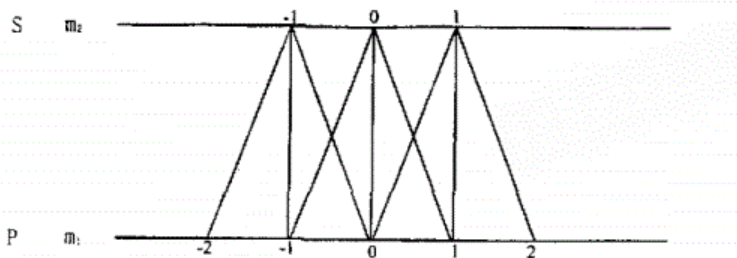
\includegraphics[width=0.4\linewidth]{汞格伦春图.png}
	
\end{figure}
\begin{question}
	请回答什么是“反常塞曼效应”和“正常塞曼效应”,两者之间的区别是什么。请思考
	什么是“帕邢-巴克效应”及其形成的原因。
\end{question}
\subsection*{正常塞曼效应 }

正常塞曼效应是指当原子在外加磁场中时,光谱线会分裂成几条新的谱线。具体分裂关系如下:

\begin{equation}
\hbar\omega' = \hbar\omega + \mu_B g (m_1 - m_2)
\end{equation}

其中,
\begin{itemize}
  \item $\hbar\omega$ 是无磁场时的光子能量,
  \item $\mu_B$ 是玻尔磁子,
  \item $g$ 是朗德g因子,在正常塞曼效应中取1,
  \item $m_1$ 和 $m_2$ 是两个能级的磁量子数。
\end{itemize}

在这种情况下,光谱线分裂为3条:一条未偏移的谱线和两条对称偏移的谱线,符合选择定则 $\Delta m = 0, \pm 1$。

\subsection*{反常塞曼效应 }

反常塞曼效应考虑了电子自旋的影响。当原子在外加磁场中时,电子的自旋和轨道角动量耦合,导致 $g$ 因子的不同,并且能级分裂更复杂。分裂关系如下:

\begin{equation}
\hbar\omega' = \hbar\omega + \mu_B (m_1 g_1 - m_2 g_2)
\end{equation}

由于自旋的不同,$g$ 因子不再恒为1,而是依赖于自旋和轨道角动量的具体情况。这可能导致多条谱线的分裂,而不是简单的3条。

\subsection*{帕邢-巴克效应 }

帕邢-巴克效应描述了在极强磁场下的塞曼效应。当外加磁场强到一定程度时,电子的轨道角动量和自旋角动量不再耦合为一个总角动量 $J$,而是分别沿着磁场方向进动。此时,各自的 $g$ 因子变得无关紧要,塞曼效应回到了类似于正常塞曼效应的情况,但能级的分裂变得简单和可预测。

\subsection*{总结}

\begin{itemize}
  \item \textbf{正常塞曼效应}:在外加磁场下,由于电子自旋影响可以忽略,能级简单地分裂成3条谱线。
  \item \textbf{反常塞曼效应}:考虑电子自旋影响,能级分裂更复杂,可能产生多条谱线。
  \item \textbf{帕邢-巴克效应}:在极强磁场下,轨道角动量和自旋角动量分离,塞曼效应回到类似正常塞曼效应的情况。
\end{itemize}


\begin{question}
	请回答电子的“自旋-轨道耦合” 的本质是什么?它与电子之间的“LS 耦合” 的区别是什么?
\end{question}

电子的“自旋-轨道耦合” 本质上是电子自旋角动量在电子绕核运动产生的磁场相互作用的效应,可以产生的能及分裂;电子的“LS 耦合” 是指电子的自旋角动量与轨道角动量进行角动量叠加,产生新的总角动量与状态空间,本质上不是与自磁场相互作用。
\begin{question}
	请结合多电子原子以及电子组态相关知识,思考为什么像汞原子一样有两个价电子的元素(He、Mg 等第二主组元素)会有两套不同的谱线(一条是单线结构,一套是双线结构) 。
\end{question}
第二主族元素的电子组态为$s^2$即两个同科 s 电子。原子组态由两个同科 s 电子耦合产生。

\begin{question}
	设 F-P 标准具两反射面之间的距离为 d=2 mm,请根据(47)式估计汞原子 546.1nm 谱
	线的自由光谱范围。
	
\end{question}
$$\Delta\lambda\approx\frac{\lambda^2}{2nd}\text{ 代入}d=2mm,\lambda=546.1nm$$$$\Delta\lambda\approx74.56pm$$

\begin{question}
	请根据(38)式,估计在外磁场为B=1T 时观察汞原子 546.1nm 谱线分离所要求的仪器分辨率的$\frac\lambda{\Delta\lambda}$,并讨论用 F-P 标准具观测的必要性(一般棱镜摄谱仪的理论分辨率为$10^3 \sim 10^4$F-P 标准具的理论分辨率为 $10^5 \sim 10^7$实际分辨率比理论值要略低一些。)
\end{question}
一般棱镜摄谱仪的理论分辨率为\(10^3 \sim 10^4\),F-P 标准具的理论分辨率为\(10^5 \sim 10^7\)。实际分辨率比理论值要略低一些。根据塞曼效应实验原理,汞原子 546.1nm 谱线分裂\(\Delta\lambda=\lambda^2\Delta\nu\approx10^{-11}\),分辨率\(\frac{\lambda}{\Delta\lambda}=5.5\times10^4\),超出一般棱镜摄谱仪的分辨率。F-P 标准具的理论分辨率为\(10^5-10^7\),实际分辨率比理论值要略低一些,故其分辨率可以包含\(5.5\times10^4\),满足实验要求。
\begin{question}
	仔细观察垂直磁场方向观察,旋转偏振片至 45°角的纪录,会发现同一级条纹在磁场中
	分离成不只二条,请解释出现这一现象的原因,
\end{question}
在磁场中观察垂直磁场方向的光学现象时,使用偏振片会导致光的偏振方向发生改变,从而导致观察到的条纹数量发生变化。

如果加上的偏振片偏振方向与$\pi$线偏振平行,那么只有$\pi$偏振光能通过偏振片,因此只能观察到3条$\pi$偏振光分裂的条纹。

如果加上的偏振片偏振方向与$\pi$线偏振垂直,那么$\sigma^+,\sigma^-$偏振光都能通过偏振片,但由于它们的偏振方向不同,分别与偏振片的偏振方向夹角为45°,因此观察到的谱线数量为6条(每个$\sigma^+,\sigma^-$各3条)。

当偏振片的偏振方向与$\pi$线偏振方向呈45°时,$\pi$偏振光和$\sigma^+,\sigma^-$偏振光都能通过偏振片,因此可以观察到全部9条谱线。

这种现象的原因在于不同偏振方向的光在通过偏振片后受到的衍射效应不同,导致在观察屏幕上出现不同数量的条纹。







\begin{question}
	请尝试计算钠双黄线(又称“钠D线”,是由钠原子从$^2P_{1/ 2, 3/ 2}\text{到 }^2S_{1/ 2}$态 的 跃 迁 所 产 生 ) 谱 线 的 
	塞曼分裂(如图 21),可能的话,设计具体实验步骤并进行观察验证。
\end{question}
这三个原子态的量子数以及各自的$g$因子如下:
$$^2P_{1/2}\colon L=1\:,S=\frac{1}{2}\:,J=\frac{1}{2}\:,g=\frac{2}{3}$$$$^2P_{3/2}\colon L=1\:,S=\frac{1}{2}\:,J=\frac{3}{2}\:,g=\frac{4}{3}$$
$$^2S_{1/2}\colon L=0,S=\frac12,J=\frac12,g=\frac63$$
根据塞曼效应能级分裂公式:
$$\hbar\omega'=\hbar\omega+\mu_BB_z(m_1g_1-m_2g_2)$$
综合选择定则:$\Delta m=0$,±1,可以得到如下图所示的可能谱线:
\begin{figure}[{H}]
	\centering
	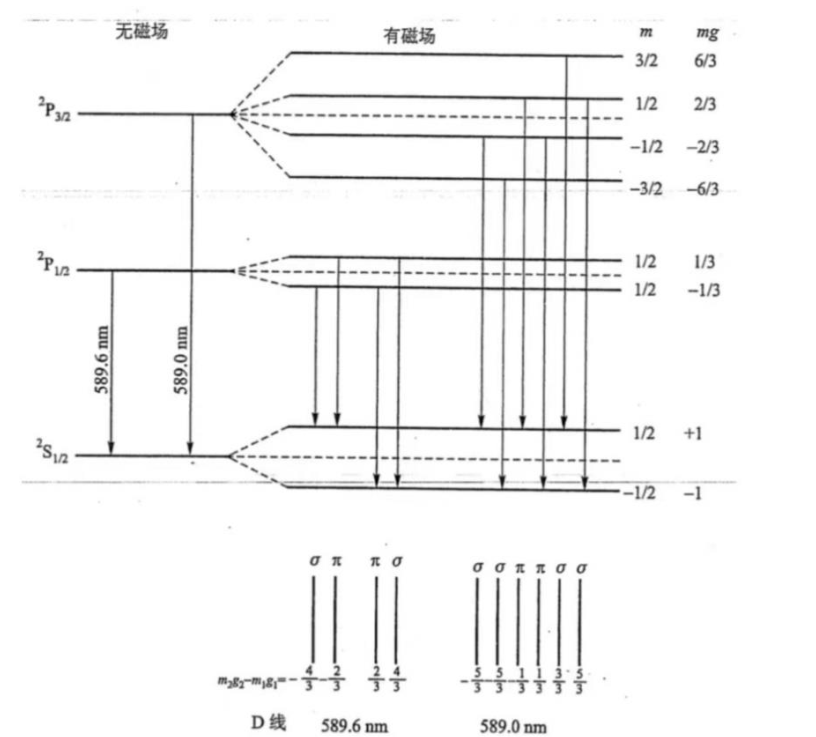
\includegraphics[width=0.6\linewidth]{钠双黄线.png}
	
	\label{}
\end{figure}
分裂得到的谱线的$(m_1g_1-m_2g_2)$因子汇总如下:
$\pi$线:士$\frac13,\pm\frac23$,总共 4 条;

$\sigma^+$线:$\frac33,\frac43,\frac53$,总共 3条;

$\sigma^-$线:$-\frac33,-\frac43,-\frac53$,总共 3 条。

实验观察Na双黄线的塞曼效应可以仿照本实验,将钠灯放置于磁场中,然后借助偏振片,分别于垂直于磁场方向、平行于磁场方向观察。下面对实验结果做出预测:

垂直于磁场方向观察:4 条$\pi$线偏振光分裂,3 条$\sigma^+$圆偏振光分裂(但是由于观察方向原因,看到的
是线偏振),3 条$\sigma^-$圆偏振光分裂(但是由于观察方向原因,看到的是线偏振)。

平行于磁场方向观察:看不到$\pi$线偏振光,但是其它 6 条光线可以看到。

	% 实验记录	
	\clearpage
	
	% 顶栏
	\begin{table}
		\renewcommand\arraystretch{1.7}
		\centering
		\begin{tabularx}{\textwidth}{|X|X|X|X|}
			\hline
			专业: & 物理学 & 年级: & 2022级 \\
			\hline
			姓名: & 黄罗琳、徐靖博 & 学号: & 22344001、22344004\\
			\hline
			室温: & 26℃ & 实验地点: & A522 \\
			\hline
			学生签名:&  & 评分: &\\
			\hline
			实验时间:& 2024/6/6 & 教师签名:&\\
			\hline
		\end{tabularx}
	\end{table}
	% ---
	
	% 小标题
	\section{塞曼效应 \quad\heiti 实验记录}
	% ---
	
	% 实验过程记录
	\subsection{实验内容、步骤与结果}
	
	%
	\subsubsection{操作步骤记录}
	\begin{enumerate}
		\item 准备工作
		\begin{enumerate}
		\item 确保电源线和相机 USB 线连接正确后,打开电源按钮,检查电流是否为
		零,汞灯是否工作正常。
		\item 打开桌面上或 D 盘的塞曼效应文件夹中的 Capstone 软件模板,点击视频
		记录或拍照功能中的预览相机按钮,通过视频窗口实时观察采集到的图像。注意
		将视频记录分辨率调至最高。
	\end{enumerate}	
		\item 光路调整(先取下光学导轨上所有光学器件)
		\begin{enumerate}
			\item 调整相机模块:将相机固定在光学导轨上的另一端约 520 mm 处,并锁紧
		托板。松开升降 调节架的螺钉,调整杆的高度,并通过旋转来微调升降调节架,
		确保相机与汞灯处于同一高度,此时汞灯图像位于屏幕中心。调节镜头上的焦距
		和光圈,使图像清晰。
		\item 调整聚光透镜和偏振片模块:将聚光透镜和偏振片固定在相机右侧的导轨
		上,并以同样方法调节高度,此时光斑将充满整个视频窗口。松开偏振片旋钮,
		旋转偏振片,使竖直白色刻度对准 90°刻线。
		\item 调节 F-P 标准具和干涉滤光片模块:将干涉滤光器和 F-P 标准具置于相机和偏振片之间,调节高度一致,并使标准具尽可能靠近相机镜头(避免杂散光),此时视频窗口会出现干涉圆环。适当调节聚光透镜的位置和相机镜头光圈,使得图像亮度适中。调节精密调整架的 XY 旋钮,使得干涉圆环处于视频窗口中心。
		调节相机镜头后焦,获得清晰干涉图像。

	\end{enumerate}	
	\item 观察谱线分裂
	调节电磁场的驱动电流并观察干涉圆环的分裂现象,如图 16。当电流大于 4A 时,
	即能观察到谱线分裂现象,当 5A 时最为清晰。
	\item 计算荷质比
	\[
				\frac{e}{m} = \frac{4\pi c}{n d B}(\frac{D^2_\alpha - D^2_K}{D^2_{K-1} - D^2_{K}})
			\]
			在磁场横向(垂直)方向上观察,分别旋转偏振片至 0°和 45°。记录
此时干涉条纹的变化,试着分析变化的原因。
\item 在平行于磁场方向,根据示意图旋转实验装置
当整套装置调整完毕,旋转偏振器 0°,45°,90°没有任何影响,说明此时的光线为圆偏正。
\subsection{垂直于磁场}
\end{enumerate}	
	
	\begin{figure}[H]
		\begin{minipage}[b]{0.3\linewidth}
		  \centering
		  \includegraphics[width=\linewidth]{1.45°.png}
		  \caption{偏振片45°,九条谱线}
		\end{minipage}
		\hfill
		\begin{minipage}[b]{0.3\linewidth}
		  \centering
		  \includegraphics[width=\linewidth]{1.0°.png}
		  \caption{偏振片0°,六条谱线}
		\end{minipage}
		\hfill
		\begin{minipage}[b]{0.3\linewidth}
		  \centering
		  \includegraphics[width=\linewidth]{1.90°.png}
		  \caption{偏振片90°,三条谱线}
		\end{minipage}
	\end{figure}
	\subsection{平行于磁场}
\begin{figure}[H]
	\begin{minipage}[b]{0.3\linewidth}
	  \centering
	  \includegraphics[width=\linewidth]{2.0°.png}
	  \caption{偏振片0°}
	\end{minipage}
	\hfill
	\begin{minipage}[b]{0.3\linewidth}
	  \centering
	  \includegraphics[width=\linewidth]{2.45°.png}
	  \caption{偏振片45°}
	\end{minipage}
	\hfill
	\begin{minipage}[b]{0.3\linewidth}
	  \centering
	  \includegraphics[width=\linewidth]{2.90°.png}
	  \caption{偏振片90°}
	\end{minipage}
\end{figure}	
\subsection{实验数据}

\begin{table}[!ht]
    \centering
    \begin{tabular}{|l|l|l|l|l|l|}
    \hline
        测量次数 & Dk1 & DK-1 & Dk & e/m & 相对误差  \\ \hline
        1 & 0.55032 & 0.98356 & 0.59584 & 1.61379E+11 & -8.20\%  \\ \hline
        2 & 0.55116 & 0.97852 & 0.59834 & 1.70526E+11 & -3.00\%  \\ \hline
        3 & 0.5443 & 0.98512 & 0.59032 & 1.59194E+11 & -9.45\%  \\ \hline
        4 & 0.53104 & 1.00432 & 0.58458 & 1.68961E+11 & -3.89\%  \\ \hline
        平均 & 0.54421 & 0.98738 & 0.59277 & 1.67201E+11 & -4.89\%  \\ \hline
        标准差 & 0.009293214 & 0.011316112 & 0.006124497 & ~ &   \\ \hline
    \end{tabular}
\end{table}


	% 问题记录
	\subsection{实验过程遇到问题及解决办法}
	\begin{enumerate}
		\item 
	\end{enumerate}
	% ---
	
	
	
	% 分析与讨论	
	\clearpage
	
	% 顶栏
	\begin{table}
		\renewcommand\arraystretch{1.7}
		\begin{tabularx}{\textwidth}{|X|X|X|X|}
			\hline
			专业:& 物理学 &年级:& 2022级\\
			\hline
			姓名: & 黄罗琳、徐靖博 & 学号:&22344001、22344004 \\
			\hline
			日期:& 2024/6/6 & 评分: &\\
			\hline
		\end{tabularx}
	\end{table}
	% ---
	
	% 小标题
	\section{塞曼效应\quad\heiti 分析与讨论}
	% ---
	
	% 数据处理
	\subsection{实验数据分析}
	\subsubsection{分析塞曼分裂情况}

		\begin{itemize}
			\item 首先在磁场垂直方向上观察,将观察到三个偏振光,$\sigma^+$左旋偏振光和$\sigma^-$右旋偏振光的投影和$\pi$偏振光,$\sigma^+$左旋偏振光和$\sigma^-$右旋偏振光的投影与磁场方向$B$垂直,$\pi$偏振光与磁场$B$平行。
			
				\begin{enumerate}
					\item 电流3.3A,偏振片90°时,如图2所示,谱线分裂为3条,只有一个线偏振光透过偏振片,综合偏振片置于0°时的图像分析,该线偏振光为$\pi$偏振光。
					\item 电流3.3A,偏振片0°时,如图3所示,谱线明显的分为两份圆环,且每份圆环还分裂为较模糊的三条谱线,谱线总共分裂为6条,此时透过0°偏振片的是$\sigma^+$左旋偏振光和$\sigma^-$右旋偏振光的投影。
					\item 电流3.3A,偏振片45°时,如图1所示,三个线偏振光都有通过,谱线应分裂为九条,但因为仪器有误差(此处误差分析见实验误差定性分析),导致有两条重叠,实际中只观察到6条。
					
				\end{enumerate}

			\item 然后在磁场平行方向上观察,将观察到两个圆偏振,$\sigma^+$左旋偏振光和$\sigma^-$右旋偏振光。
				
				\begin{enumerate}
					\item 基于实验原理和他人实验图像,可以观察出在磁场的影响下,应为6条谱线,我们实验图像的确在90°时观察出六条谱线(图7)
					\item 电流为3.3A,如图5-7,正常来说,现在为圆偏振光,不应随着旋转偏振片而出现变化,但是实际上的确出现了变化,但是变化并不是实验图像出现了圆环半径的变化,而是在两个分裂导致的六条分裂谱线更加清晰了。
					\item 谱线分裂为两条粗环,分别代表$\sigma^+$左旋偏振光和$\sigma^-$右旋偏振光。
				\end{enumerate}
		\end{itemize}
	%
	\subsubsection{实验误差定性分析}
	\begin{enumerate}
		\item 对于实验所显示的实验图像,误差主要体现在显示的谱线明显非常模糊,并且出现了上半部分相比于下半部分更加模糊的情况,初步分析主要为实验光路的问题,实验光路的调整不当,导致了尽管出现了正确的实验结果但是因为光路问题无法争取的在屏幕上进行读取。
		\item 对于磁场平行方向上的观察出现的不同于理论和实验预测的结果(偏振片旋转导致了实验图像变化),首先尽管实验图像发生了变化,但是两个较清晰的圆并没有发生变化,发生变化的是两圆间的区域,这片区域出现的变化导致了符合实验另一个预期(6条谱线)的现象出现,这说明这部分并不是错误的实验图像,初步判断这部分实验图像的变化是由于光路的调整不当导致的。
		\item 对于实验数据的读取和计算误差,这部分误差主要是由于,我们尽管可以在实验图像中进行数据提取,但是我们明显可以看出,圆环存在一定的宽度,这可能导致在读取的时候存在读取的主观性(何处为直径结束点,何处为直径),并且在实验仪器中进行三点画圆的步骤,这三个点的选取也会出现误差,圆心可能并不是图像的圆心,这一系列都会导致实验的数据出现误差。
	\end{enumerate}
	
	%
	\subsubsection{实验误差定量分析}
	误差传递公式为:\[
			\sigma_{\frac{e}{m}} = \sqrt{\left(\frac{\partial\left(\frac{e}{m}\right)}{\partial D_{K1}} \cdot \sigma_{D_{K1}}\right)^2 + \left(\frac{\partial\left(\frac{e}{m}\right)}{\partial D_K} \cdot \sigma_{D_K}\right)^2 + \left(\frac{\partial\left(\frac{e}{m}\right)}{\partial D_{K-1}} \cdot \sigma_{D_{K-1}}\right)^2}
		\]
	
	\[
			\frac{\partial\left(\frac{e}{m}\right)}{\partial D_k} = 29235304771
		\]

		\[
			\frac{\partial\left(\frac{e}{m}\right)}{\partial D_{k1}} =  2766906464
		\]

		\[
			\frac{\partial\left(\frac{e}{m}\right)}{\partial D_{K-1}}  = -3730944971
		\]

		可得间接测量量$e/m$的标准差为:

		\[
			\begin{aligned}
			\sigma_{e/m} &= \sqrt{(29235304771 \times 0.180773994)^2 + (2766906464 \times 0.372637827)^2 + (-3730944971 \times 0.473122503)^2 } \\
			&= 5666570886 = 5.67 \times 10^9
			\end{aligned}
		\]


		展伸不确定度$U = k \sigma_{e/m}$,置信概率取95 \% 时,$k = 1.96$,则$U = k \sigma_{e/m} = 1.11 \times 10^{10}		$
		
		则最后测量结果为:$e/m = (1.92 \pm 0.11) \times 10^{11} C \cdot kg$

	\subsubsection{}
	
	% ---
	

	
	
	% 结语部分
	\clearpage
	
	% 小标题
	\section{塞曼效应\quad\heiti 结语}
	% ---
	
	% 总结、杂谈与致谢
	\subsection{实验心得和体会、意见建议等}
	\begin{enumerate}
		\item 实验整体难度在于如何调整出正确的实验图像,其大部分操作和误差引入都是因为仪器和光路的调整问题。
		\item 对于实验的图像输出,尽管我通过后期的代码拟合
	\end{enumerate}
	% ---
	

	% 附件
	\subsection{附件及实验相关的软硬件资料等}
	试验台桌面整理如%\cref{}所示。
	
	实验报告个人签名如

	% ---
	
	
\end{document}